\documentclass[tikz, border=10pt]{standalone}
\usetikzlibrary{calc, decorations.pathreplacing, patterns}

\begin{document}
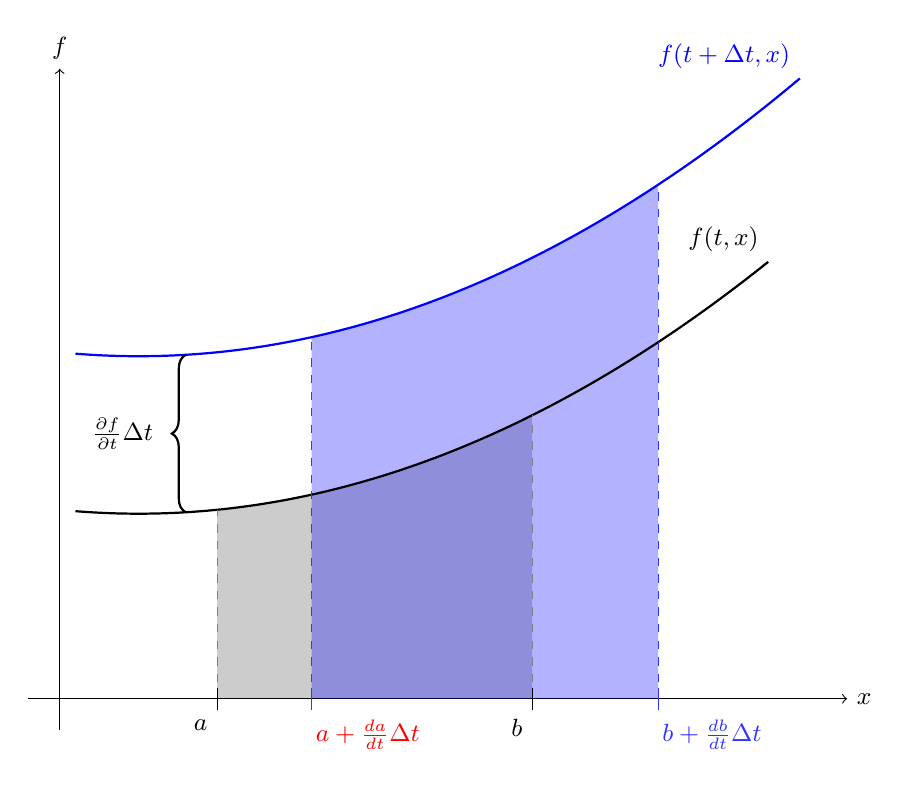
\begin{tikzpicture}[
    scale=2.0,
    important line/.style={thick},
    dashed line/.style={dashed, thin, gray},
    every node/.style={font=\small},
    base area/.style={fill=black, fill opacity=0.2},
    shifted area/.style={fill=blue, fill opacity=0.3}
]
    % Axes
    \draw[->] (-0.2,0) -- (5.0,0) node[right] {$x$};
    \draw[->] (0,-0.2) -- (0,4.0) node[above] {$f$};

    % Definitions & Variables
    \def\a{1.0}
    \def\da{0.6}
    \pgfmathsetmacro{\anew}{\a + \da}
    
    \def\b{3.0}
    \def\db{0.8}
    \pgfmathsetmacro{\bnew}{\b + \db}
    
    \def\shiftY{1.0}
    \def\xLeft{0.8} % <-- Decreased value moves the brace left

    % Calculated Functions
    \pgfmathdeclarefunction{funcF}{1}{\pgfmathparse{0.1*#1*#1 - 0.1*#1 + 1.2}}
    \pgfmathdeclarefunction{funcFdt}{1}{\pgfmathparse{0.1*#1*#1 - 0.1*#1 + 1.2 + \shiftY}}

    % Shaded Areas
    \fill[base area] (\a,0) -- plot[domain=\a:\b, samples=100] (\x, {funcF(\x)}) -- (\b,0) -- cycle;
    \fill[shifted area] (\anew,0) -- plot[domain=\anew:\bnew, samples=100] (\x, {funcFdt(\x)}) -- (\bnew,0) -- cycle;

    % Curves (Domain starts at 0.1 now to connect with the moved brace)
    \draw[important line] plot[domain=0.1:4.5, samples=100] (\x, {funcF(\x)});
    \draw[important line, blue] plot[domain=0.1:4.7, samples=100] (\x, {funcFdt(\x)});

    % Curve Labels
    \node[above left] at (4.5, {funcF(4.5)}) {$f(t,x)$};
    \node[above left, blue] at (4.7, {funcFdt(4.7)}) {$f(t+\Delta t, x)$};

    % Boundary Projections
    \draw[dashed line] (\a,0) -- (\a, {funcF(\a)});
    \draw[dashed line] (\b,0) -- (\b, {funcF(\b)});
    \draw[dashed line, red] (\anew,0) -- (\anew, {funcFdt(\anew)});
    \draw[dashed line, blue!80] (\bnew,0) -- (\bnew, {funcFdt(\bnew)});

    % X-Axis Marks & Direct Labels
    \draw (\a, 2pt) -- (\a, -2pt) node[below left] {$a$};
    \draw[red] (\anew, 2pt) -- (\anew, -2pt) node[below right, xshift=-2pt] {$a + \frac{da}{dt}\Delta t$};
    
    \draw (\b, 2pt) -- (\b, -2pt) node[below left] {$b$};
    \draw[blue!80] (\bnew, 2pt) -- (\bnew, -2pt) node[below right, xshift=-2pt] {$b + \frac{db}{dt}\Delta t$};

    % Vertical Brace 
    \pgfmathsetmacro{\fxL}{funcF(\xLeft)}
    \pgfmathsetmacro{\fxdtL}{funcFdt(\xLeft)}
    \draw[decorate, decoration={brace, amplitude=5pt}, thick] 
        (\xLeft, \fxL) -- (\xLeft, \fxdtL) 
        node[midway, left=8pt] {$\frac{\partial f}{\partial t}\Delta t$};

\end{tikzpicture}
\end{document}